\chapter{Implementace}
Tato kapitola se zabývá procesem implementace nové webové aplikace. Nejdříve budou představeny nástroje, které jsem při vývoji využíval, a bude popsána struktura projektu. Následně budou přiblíženy vybrané části implementace a nakonec budou diskutovány další možná rozšíření.

\section{Použité nástroje}


\section{Struktura projektu}
Projekt následuje standardní adresářovou strukturu Symfony aplikací a tedy orientace by lidem, kteří se již s nějakou aplikací vytvořenou v Symfony frameworku setkali, neměla dělat problém.

\dirtree{%
    .1 .
    .1 config\DTcomment{konfigurační soubory aplikace}.
    .1 public\DTcomment{kaskádové styly, kód v jazyku JavaScript, ikony}.
    .1 src.
    .2 Controller\DTcomment{controllery}.
    .2 Form\DTcomment{formuláře}.
    .2 Entity\DTcomment{modely}.
    .1 templates\DTcomment{šablony stránek}.
    .1 composer.json\DTcomment{soubor se seznamem závislostí}.
}

\section{Ukázky vybraných částí}
V následující sekci je popsáno několik vybraných částí z implementované aplikace, které jsou pro~vytvořený systém důležité nebo jsou nějakým způsobem zajímavé. Jako první bude představen způsob komunikace s informačním systémem Českého svazu orietačních sportů ORIS, poté bude popsána tvorba formuláře pro přidání nové události a jako poslední bude demonstrován způsob zobrazení aplikace na různých typech klientských zařízení.

\subsection{Komunikace s IS ORIS}
Jednou z nových funkcí oproti současně používanému systému je napojení na IS ORIS. Konkrétně je v nové aplikaci umožněno automatické načítání informací o závodu evidovaného v celorepublikovém systému a také odesílání evidovaných přihlášek. Propojení je dosaženo s využitím dostupného API, které je popsáno v sekci \ref{implementation:oris-api}.

\subsubsection{Webové API}\label{implementation:api}
Zkratku API lze do češtiny přeložit jako „rozhraní pro programování aplikací“. Z tohoto slovního spojení však člověk, který se v oblasti informačních technologií nepohybuje, pravděpodobně stále nebude mít moc představu, k čemu to API vlastně je. V případě webových aplikací se jedná o rozhraní, které umožňuje komunikaci mezi různými systémy nebo různými částmi systému. Jedna strana musí toto rozhraní, jež se může skládat z více koncových bodů (endpointů), poskytovat a druhá následně může na některý z těchto endpointů posílat povolené instrukce, a tím s první interagovat. V dnešní době je pro API orientovaná na data nejčastěji využívána architektura REST, avšak informační systém ORIS své API založil na vlastní architektuře, jejíž popis je součástí následující sekce \ref{implementation:oris-api}. \cite{api}

\subsubsection{ORIS API}\label{implementation:oris-api}
Veškerá komunikace s ORIS API probíhá pomocí GET požadavků. Každý požadavek musí obsahovat query parametr s názvem metody a názvem formátu, ve kterém chceme data obdržet. V závislosti na vybrané metodě může být nutné uvést i další query parametry, které jsou pro~ni specifické. V současné době je podporováno 28 různých method a 2 datové formáty (JSON a XML). Příklad požadavku na získání všech klubů v Českém svazu orientačních sportů ve formátu JSON můžeme vidět na výpisu kódu \ref{listing:api}. 

\begin{listing}[h]
    \caption{Požadavek na získání všech klubů v ČSOS}\label{listing:api}
    \begin{minted}{http}
GET /API/?format=json&method=getCSOSClubList HTTP/1.1
Host: oris.orientacnisporty.cz
Accept: */*
    \end{minted}
\end{listing}

V nové aplikaci jsou využity 4 z nabízených metod. Konkrétně se jedná o metody \mintinline{text}|getEvent|, \mintinline{text}|getEventList|, \mintinline{text}|getRegistration| a \mintinline{text}|createEntry|. Metoda \mintinline{text}|getEvent| se využívá pro načtení informací o závodě při vytváření nové události, \mintinline{text}|getEventList| se volá při hromadné kontrole času uzávěrky přihlášek a zbývající dvě metody \mintinline{text}|getRegistration| a \mintinline{text}|createEntry| se podílejí na~odesílání přihlášek do IS ORIS.

\subsubsection{Importování nového závodu}
Jak již bylo zmíněno, při přidávání nového závodu je možné využít automatické načítání informací z celorepublikového systému. Procesy vykonávané v rámci této funkcionality lze rozdělit na~4~logické fáze:
\begin{enumerate}
    \item Získání ORIS ID závodu od uživatele
    \item Odeslání požadavku na ORIS API
    \item Zpracování přijatých dat
    \item Načtení zpracovaných dat do formuláře
\end{enumerate}

V rámci první fáze uživatel vyplní vstupní pole pro ORIS ID ve formuláři a klikne na tlačítko \emph{Importovat závod}. Kliknutím na uvedené tlačítko se spustí mechanismus, který na ORIS API pošle požadavek o zaslání dat týkající se závodu s vyplněným ORIS ID. Příklad validního požadavku a následné odpovědi, je na výpisu kódu \ref{listing:get-event-request} respektive \ref{listing:get-event-response}.

\begin{listing}[h]
    \caption{Požadavek na získání informací o závodu}\label{listing:get-event-request}
    \begin{minted}{http}
GET /API/?format=json&method=getEvent&id=6734 HTTP/1.1
Host: oris.orientacnisporty.cz
Accept: */*
    \end{minted}
\end{listing}

\begin{listing}[h]
    \caption{Začátek odpovědi na požadavek na získání informací o závodu}\label{listing:get-event-response}
    \begin{minted}{http}
HTTP/1.1 200 OK
Date: Sun, 17 Apr 2022 12:06:08 GMT

    \end{minted}
    \vspace{-11mm}
    \begin{minted}{json}
{
    "Method": "getEvent",
    "Format": "json",
    "Status": "OK",
    "ExportCreated": "2022-04-17 14:06:09",
    "Data": {
        "ID": "6734",
        "Name": "Oblastní žebříček",
        "Date": "2022-04-02",
        "Place": "Lomnice nad Popelkou",
        "Map": "Tábor, 1:10000",
    \end{minted}
\end{listing}

Z přijatých dat je pomocí speciální třídy sestaven nový objekt typu \mintinline{text}|Race|, jenž je následně předán formuláři. Ten si již jen načte data z tohoto objektu a výsledná stránka včetně předvyplněných hodnot je zaslána uživateli.

\subsubsection{Odesílání přihlášek}
TODO - dopsat po implementaci

\subsection{Formuláře}
Jednou z komplikovanějších částí implementace bylo vytvoření formulářů pro přidávání a úpravu událostí. Symfony poskytuje propracovaný systém pro práci s formuláři, který zahrnuje jejich vytváření, renderování, zpracování nebo i validaci. Součástí zpracování formuláře je i možnost jeho propojení s konkrétním objektem, díky čemuž se vyplněné hodnoty do tohoto objektu automaticky propisují. Validace vyplněných hodnot probíhá jak na straně klienta díky nastavenému atributu \mintinline{text}|type| u tagu \mintinline{text}|input|, tak na straně serveru, kde je řešena s využitím Symfony validátorů\footnote{Přesný název je „Symfony Validation Constraints“}.

Pro vlastnosti objektu \mintinline{text}|Event|, jež jsou typu \mintinline{text}|string|, \mintinline{text}|integer| nebo \mintinline{text}|datetime|, nebylo vytváření formuláře nijak speciální. Zajímavější bylo vymyslet, jakým způsobem do formuláře přidat vlastnosti \mintinline{text}|categories| a \mintinline{text}|organizers|, která jsou v databázi reprezentované vazbou M:N mezi entitami \mintinline{text}|Event| a \mintinline{text}|Category|, respektive \mintinline{text}|Event| a \mintinline{text}|Organizer|. Uvedený typ vazby M:N v případě entit \mintinline{text}|Event| a \mintinline{text}|Category| znamená, že událost může mít libovolné množství kategorií a naopak konkrétní kategorie může být přiřazena k libovolnému počtu událostí.

Po zvážení dostupných možností jsem se rozhodl vytvořit formulář, ve kterém je možné dynamicky přidávat a odebírat nové kategorie a organizátory. Nové položky lze do formuláře přidat vybráním již existujícího záznamu registrovaného u jiné události, nebo vytvořením zcela nové položky. Finální vzhled části formuláře obsahující sekci s kategoriemi je zobrazen na obrázku \ref{figure:form}.

\begin{figure}[h]
    \caption{Část formuláře na přidávání událostí}
    \label{figure:form}
    \centering
    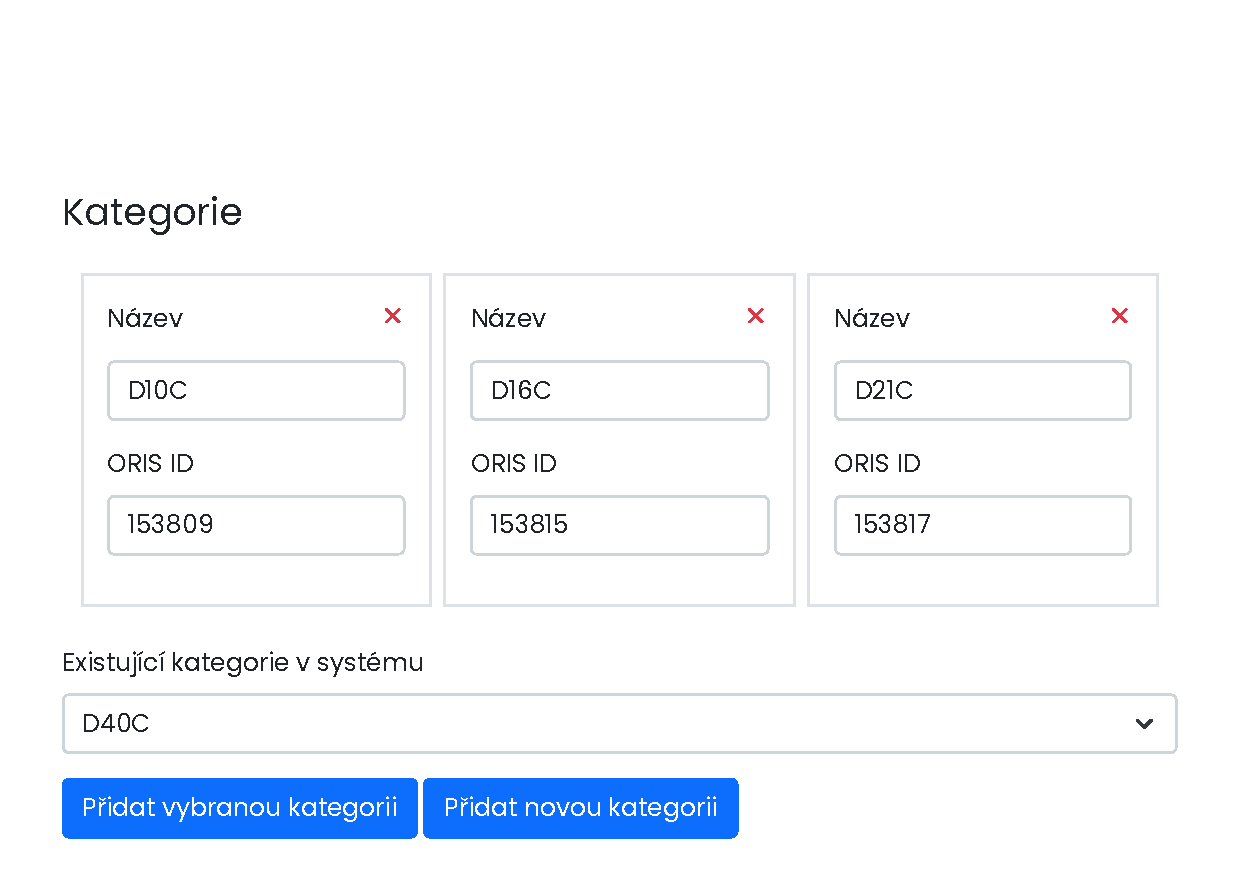
\includegraphics[width=0.95\linewidth]{images/form.pdf}
\end{figure}

Logiku ukládání a odebírání položek nebylo třeba vymýšlet od začátku, poněvadž Symfony formuláře obsahují podporu pro přidávání libovolného počtu položek ke kontrétní vlastnosti. Pro~zprovoznění této funkcionality však bylo nezbytné přidat vlastní JavaScriptový kód, který zařídí samotné přidávání a odebírání položek z objektového modelu dokumentu (DOM). V souvislosti s dynamickým přidáváním nových položek bylo nutné navíc zamezit jejich duplikování v databázi v případě shody hodnot jejich vlastností.

\subsection{Responzivní vzhled}

\section{Možná rozšíření}

